\section{Schnittstellen}
\subsection{Externe Schnittstellen}
Die folgenden externen Schnittstellen sind im Projekt enthalten:
\begin{enumerate}
	\item Logger
	\item LoggerSetup
	\item LogLevel
	\item StringPersitor
\end{enumerate}

\subsubsection{Logger}
\begin{figure}[H]
	\centering
	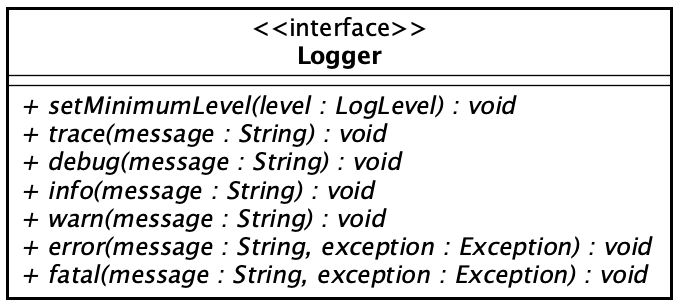
\includegraphics[width=0.5\textwidth]{3_Schnittstellen/Bilder/loggerInterface.png}
	\caption{LoggerInterface Klassendiagram}
	\label{fig:LoggerInterface Klassendiagramm}
\end{figure}
Das Logger-Interface, über welches verschiedenste Applikationen Log-Einträge erfassen können enthält insgesamt acht Methoden. Für die einzelnen Log-Levels existieren eigene Methoden. Des Weiteren enthält das Logger-Interface eine Methode zur Setzung des minimalen Log-Levels. 
\subsubsection{LoggerSetup}
\begin{figure}[H]
	\centering
	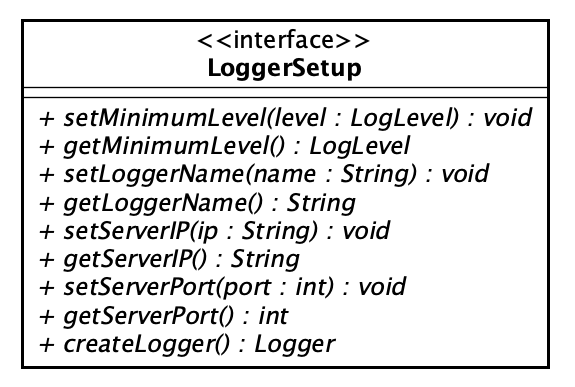
\includegraphics[width=0.5\textwidth]{3_Schnittstellen/Bilder/loggerSetupInterface.png}
	\caption{LoggerSetup Klassendiagram}
	\label{fig:LoggerSetup Klassendiagramm}
\end{figure}
Das LoggerSetup-Interface enthält neun Methoden, welche für die Erstellung eines voll funktionsfähigen Loggers benötigt werden. So muss definiert werden, wie die Server-IP-Adresse und dessen Port gesetzt werden kann. Des Weiteren kann bereits definiert werden, welcher minimale Log-Level der Logger zu Beginn besitzt. Der Logger-Name soll ebenfalls über eine Setter-Methode gesetzt werden können. Die wichtigste Methode ist die Factory-Methode createLogger, welche einen Logger vom Interfacetyp Logger zurückgeben soll.
\subsubsection{LogLevel}
\begin{figure}[H]
	\centering
	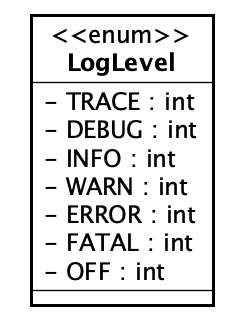
\includegraphics[width=0.2\textwidth]{3_Schnittstellen/Bilder/logLevel.png}
	\caption{Log-Level Klassendiagram}
	\label{fig:Log-Level Klassendiagramm}
\end{figure}
Die Log-Level Enumeration definiert die möglichen Log-Level, durch die klare Definition der Log-Level ist ein Austausch der Logger-Komponente möglich. Die Enumeration enthält ebenfalls einen numerischen Wert, um die Überprüfung des minimalen Log-Level möglichst einfach und performant zu gestalten.
\subsubsection{StringPersistor}
\begin{figure}[H]
	\centering
	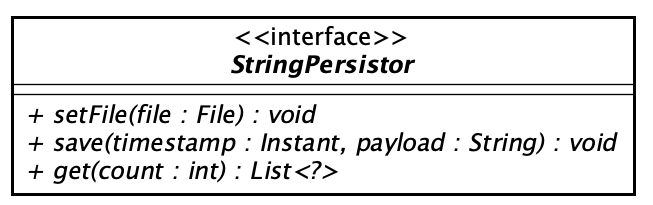
\includegraphics[width=0.5\textwidth]{3_Schnittstellen/Bilder/stringPersistorInterface.png}
	\caption{StringPersistor-Interface Klassendiagram}
	\label{fig:StringPersistor-Interface Klassendiagramm}
\end{figure}
Das StringPersistor-Interface gibt Methoden zur Speicherung von Strings in eine Datei vor. Das Format dieser Datei ist jedoch nicht durch das Interface vorgegeben. Mit der setFile()-Methode soll definiert werden, in welche Datei die Strings gespeichert werden sollen. Die tatsächliche save-Methode verlangt einen Instant-Zeitstempel und den String der gespeichert werden soll. So soll jede String-Speicherung einer Zeit zugeordnet werden können. Da es sich um ein StringPersistor-Interface handelt, existiert auch eine Methode, die eine Liste von Strings wieder zurückgeben soll.
\newpage
\subsection{Interne Schnittstellen}
Die folgenden internen Schnittstellen wurden durch das Projektteam definiert: 
\begin{enumerate}
	\item LogMessage
	\item LogPersistor
	\item TCP / IP
	\item client.properties
	\item server.properties
\end{enumerate}

\subsubsection{LogMessage}
\subsubsection{LogPersistor}
\subsubsection{TCP / IP}
\begin{figure}[H]
	\centering
	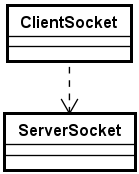
\includegraphics[width=0.2\textwidth]{3_Schnittstellen/Bilder/tcpip.png}
	\caption{TCP/IP Schnittstelle}
	\label{fig:TCP/IP Klassendiagramm}
\end{figure}
Das TCP/IP Protokoll wird verwendet, um die Kommunikation ziwschen dem ClientSocket und dem ServerSocket herzustellen. Der ServerSocket wartet in seiner listen() Methode auf einen ClientSocket und nimmt dessen Verbindung an.
\subsubsection{client.properties}
\subsubsection{server.properties}